\subsection{Case02 - Pass}
\label{xdp_wifi_case02}

En este caso de uso se probará que es posible admitir todos los paquetes recibidos haciendo uso de la tecnología \gls{xdp} en un entorno inalámbrico. ¿Qué significa ``Admitir”? se quiere comprobar si es posible dejar pasar los paquetes, sin afectarles el plano de datos programado con la tecnología, ya que, aunque \gls{xdp} mucha gente lo concibe para hacer un \textit{by-pass} al \textit{stack} de red del Kernel de Linux, una completa redefinición del mismo, en muchas ocasiones será útil trabajar en conjunto para conseguir la funcionalidad deseada. En este caso, además se verá si existe alguna diferencia inducida por el cambio de entorno, de alámbrico a \textit{wireless}.\\
\par


\vspace{0.5cm}
\textbf{Compilación}\\
\par

Para compilar el programa \gls{xdp}, al igual que en casos de uso anteriores, se ha dejado un Makefile preparado en este directorio. Por lo tanto, para compilarlo únicamente hay que seguir las indicaciones del bloque \ref{code:case02_xdp_wifi_compilacion}.\\
\par

\begin{lstlisting}[language= bash, style=Consola, caption={Compilación programa XDP - Case02},label=code:case02_xdp_wifi_compilacion]
    # En caso de no haber entrado en el directorio asignado del caso de uso
    cd TFG/src/use_cases/xdp-wireless/case02
    
    
    # Hacemos uso del Makefile suministrado 
    sudo make
\end{lstlisting}
\vspace{0.5cm}

Si tiene dudas sobre el proceso de compilación del programa \gls{xdp} le recomendamos que vuelva al case02 (\gls{xdp} - Cableado \ref{xdp_ether_case02}) donde se hace referencia al \textit{flow} dispuesto para la compilación de los programas \gls{xdp}.\\
\par



\vspace{1cm}
\textbf{Puesta en marcha del escenario}\\
\par

Para testear los programas \gls{xdp} en un entorno inalámbrico, se hará uso de Mininet-WiFi para emular las topologías de red. Para levantar el escenario solo se tendrá que ejecutar el script en Python que hace uso de la API de Mininet-WiFi para generar toda la topología de red. Una vez ejecutado este abrirá la interfaz de linea de comandos de Mininet-WiFi, desde la cual se podrá comprobar el funcionamiento del caso de uso. En este caso, se realiza la carga del programa \gls{xdp} desde el propio script de Python, haciendo uso de la herramienta xdp\_loader desarrollada para ello. Por tanto, como se ha dicho este script está auto-contenido, por lo que solo se deberá ejecutarlo. \\
\par

Para limpiar la máquina del escenario recreado anteriormente con Mininet-WiFi se podría realizar un \texttt{sudo mn -c}, pero se recomienda al usuario que haga uso del \textit{target} del Makefile destinado para ello, ya que adicionalmente limpiará los ficheros intermedios generados en el proceso de compilación de nuestro programa \gls{xdp}. Ejecutando el siguiente comando se limpiaría la máquina.\\
\par

\begin{lstlisting}[language= bash, style=Consola, caption={Compilación programa XDP - Case02},label=code:case02_xdp_wifi_run]
    # Levantamos el escenario
    sudo python runenv.py
    
    
    # Limpiamos el escenario
    sudo make clean
\end{lstlisting}
\vspace{0.5cm}


Por último, únicamente indicar que el escenario recreado es el siguiente, compuesto exclusivamente de dos estaciones \textit{wireless}, aisladas en sus propias \textit{Network Namespaces}, y un punto de acceso corriendo el \textit{daemon} de HostApd para intercomunicar dichas estaciones WiFi.\\
\par

% figura escenario
\begin{figure}[ht]
    \centering
    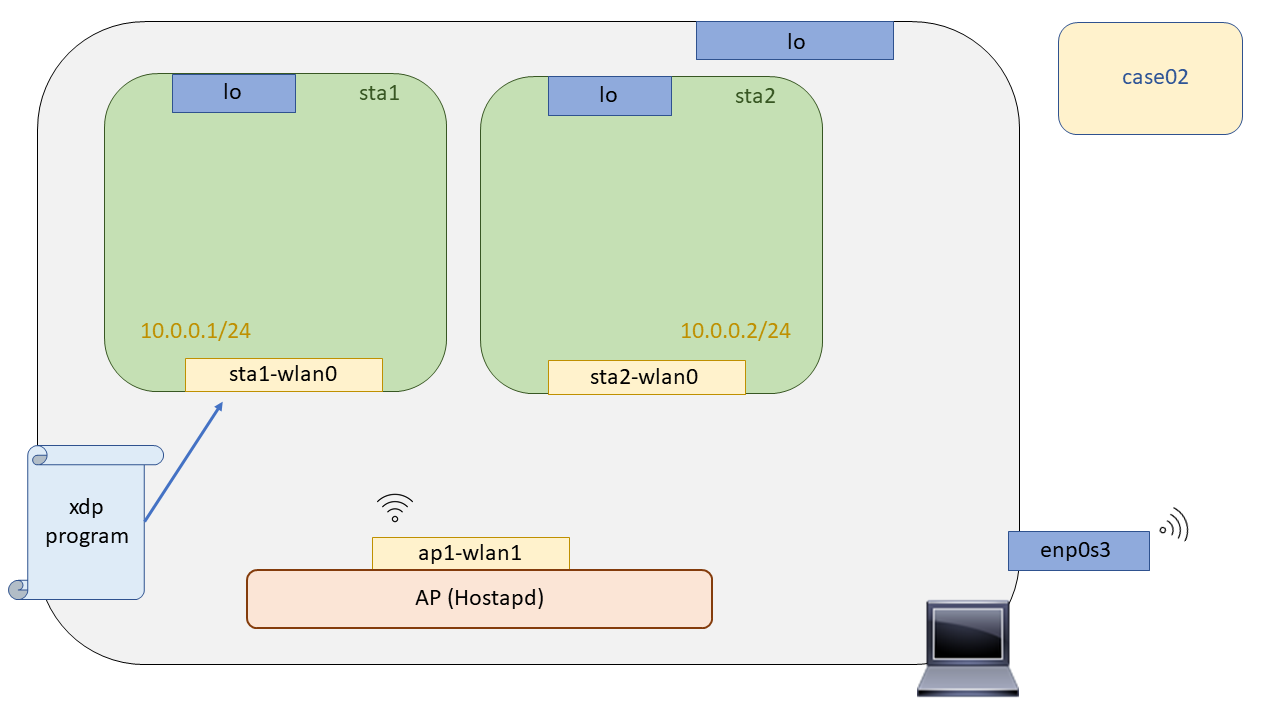
\includegraphics[width=16cm]{archivos/img/dev/xdp-wifi/case02/scenario.png}
    \caption{Escenario inalámbrico del Case02 - XDP}
    \label{fig:case02_xdp_wifi_scenario}
\end{figure}


\vspace{0.5cm}
\textbf{Carga del programa XDP}\\
\par
Como ya se ha comentado, la carga del programa \gls{xdp}, se llevará a cabo en el proceso del levantamiento del escenario, descrito en el script de Python para crear la topología. La carga del programa \gls{xdp}, se hará con el programa \texttt{xdp\_loader}, utilizado anteriormente para cargar los programas \gls{xdp} en interfaces alámbricas. \\
\par

\begin{lstlisting}[language= bash, style=Consola, caption={Carga del programa XDP - Case02},label=code:case02_xdp_wifi_load]
    # Linea 37 del script runenv.py
    sta1.cmd("./xdp_loader -S -d sta1-wlan0 -F --progsec xdp_case02")
\end{lstlisting}
\vspace{0.5cm}
En estos primeros casos de uso \gls{xdp} en un entorno inalámbrico, la carga de los programas se está realizando en el propio script que levanta la topología en Mininet-WiFi, pero más adelante en el case04 (Ir a subsección \ref{xdp_wifi_case04}) se verá como se puede ejecutar comandos dentro de la \textit{Network Namespace} indicada para lograr la carga de un programa \gls{xdp} en una interfaz de un nodo independiente de la red desde la propia CLI de Mininet-WiFi.\\
\par



\vspace{0.5cm}
\textbf{Comprobación del funcionamiento}\\
\par

Una vez que el programa \gls{xdp} fue anclado a la interfaz de la estación WiFi \texttt{sta1}, es necesario asegurarse de que funciona según lo esperado, y ver si el funcionamiento obtenido difiere al funcionamiento de este mismo caso de uso en un medio cableado.  La prueba que se va a realizar puede que sea un poco simple, pero es válida, ya que únicamente queremos verificar que el programa anclado en la interfaz está delegando los paquetes que le llegan al \textit{stack} de red.\\
\par



\begin{lstlisting}[language= bash, style=Consola, caption={Comprobación del funcionamiento - Case02},label=code:case02_xdp_wifi_func1]
    # Hacemos ping desde una estación wifi hacia la otra. Deberíamos tener conectividad.
    mininet-wifi> sta2 ping sta1
    
    # Comprobamos los códigos de retorno XDP
    mininet-wifi> sta1 ./xdp_stats -d sta1-wlan0
\end{lstlisting}

% figura escenario
\begin{figure}[ht]
    \centering
    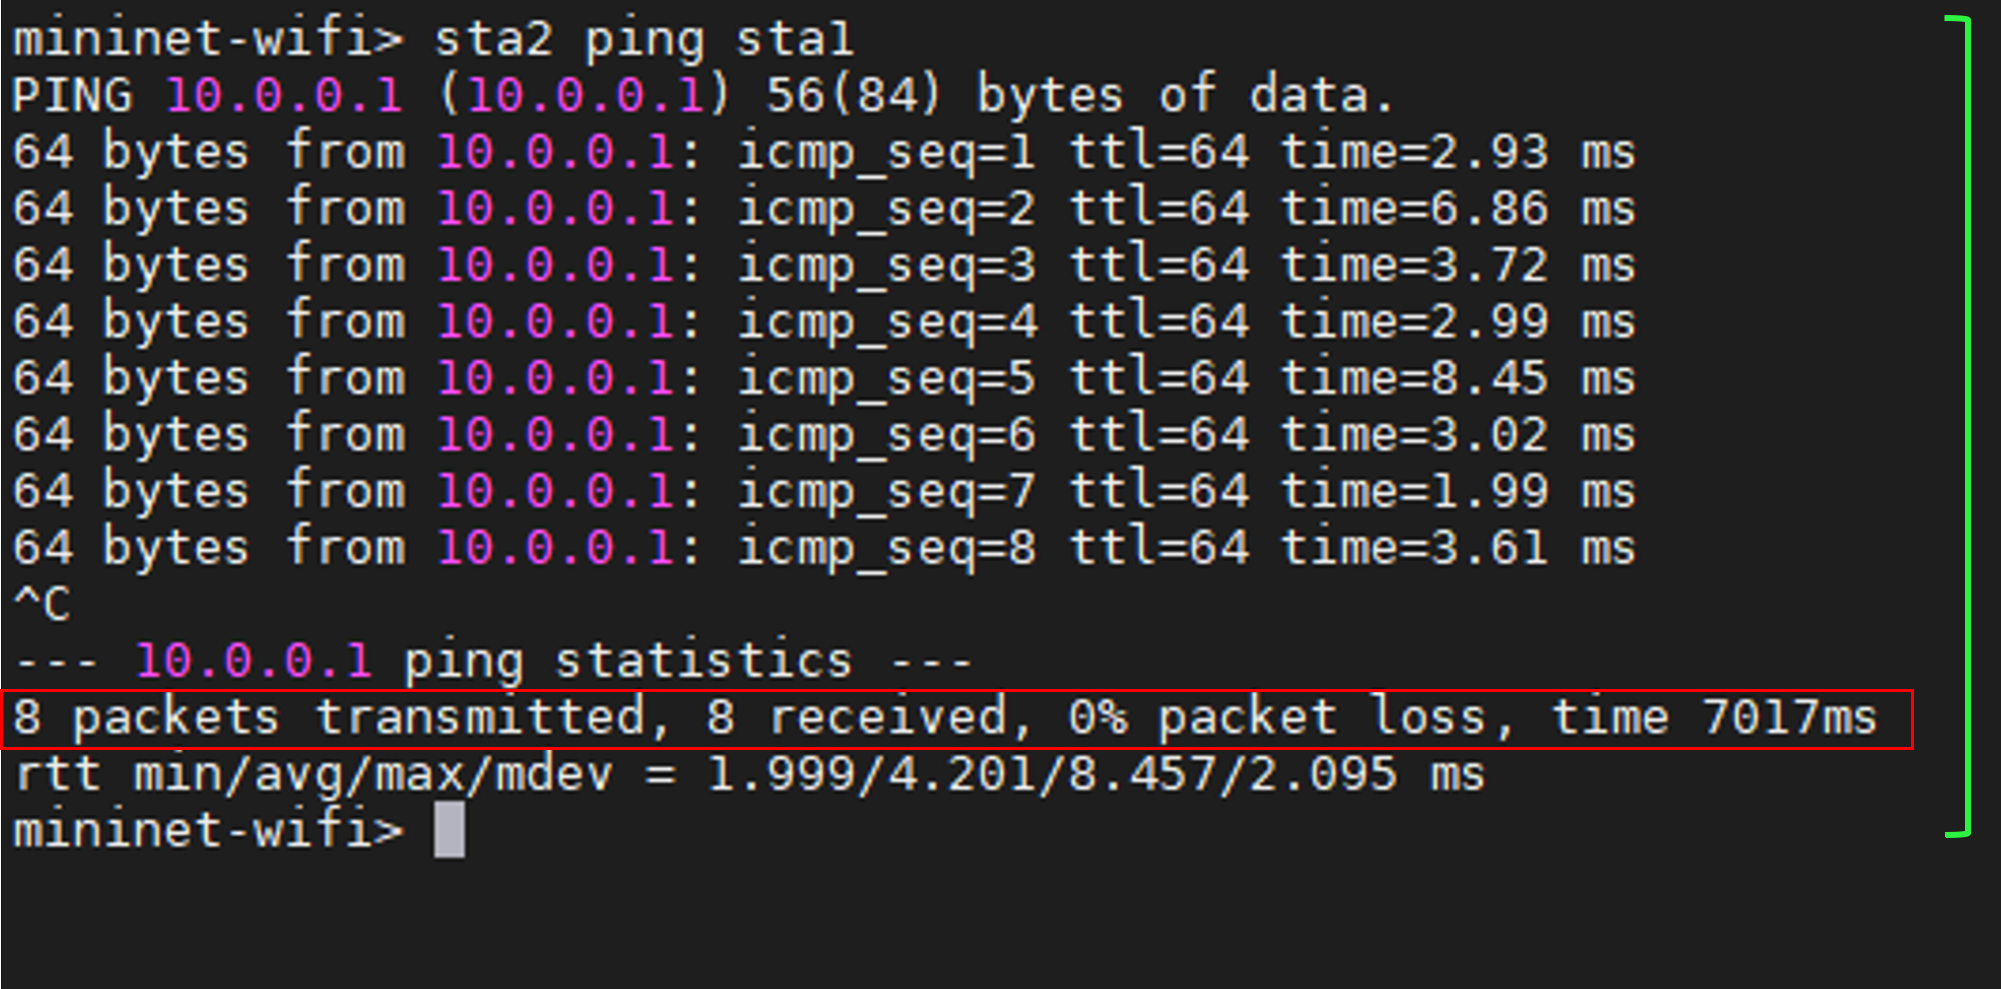
\includegraphics[width=12cm]{archivos/img/dev/xdp-wifi/case02/demo_case02_1_edited.png}
    \caption{Comprobación de funcionamiento (Ping) del Case02 - XDP Wireless}
    \label{fig:case02_xdp_wifi_func1}
\end{figure}
\newpage
% figura escenario
\begin{figure}[ht!]
    \centering
    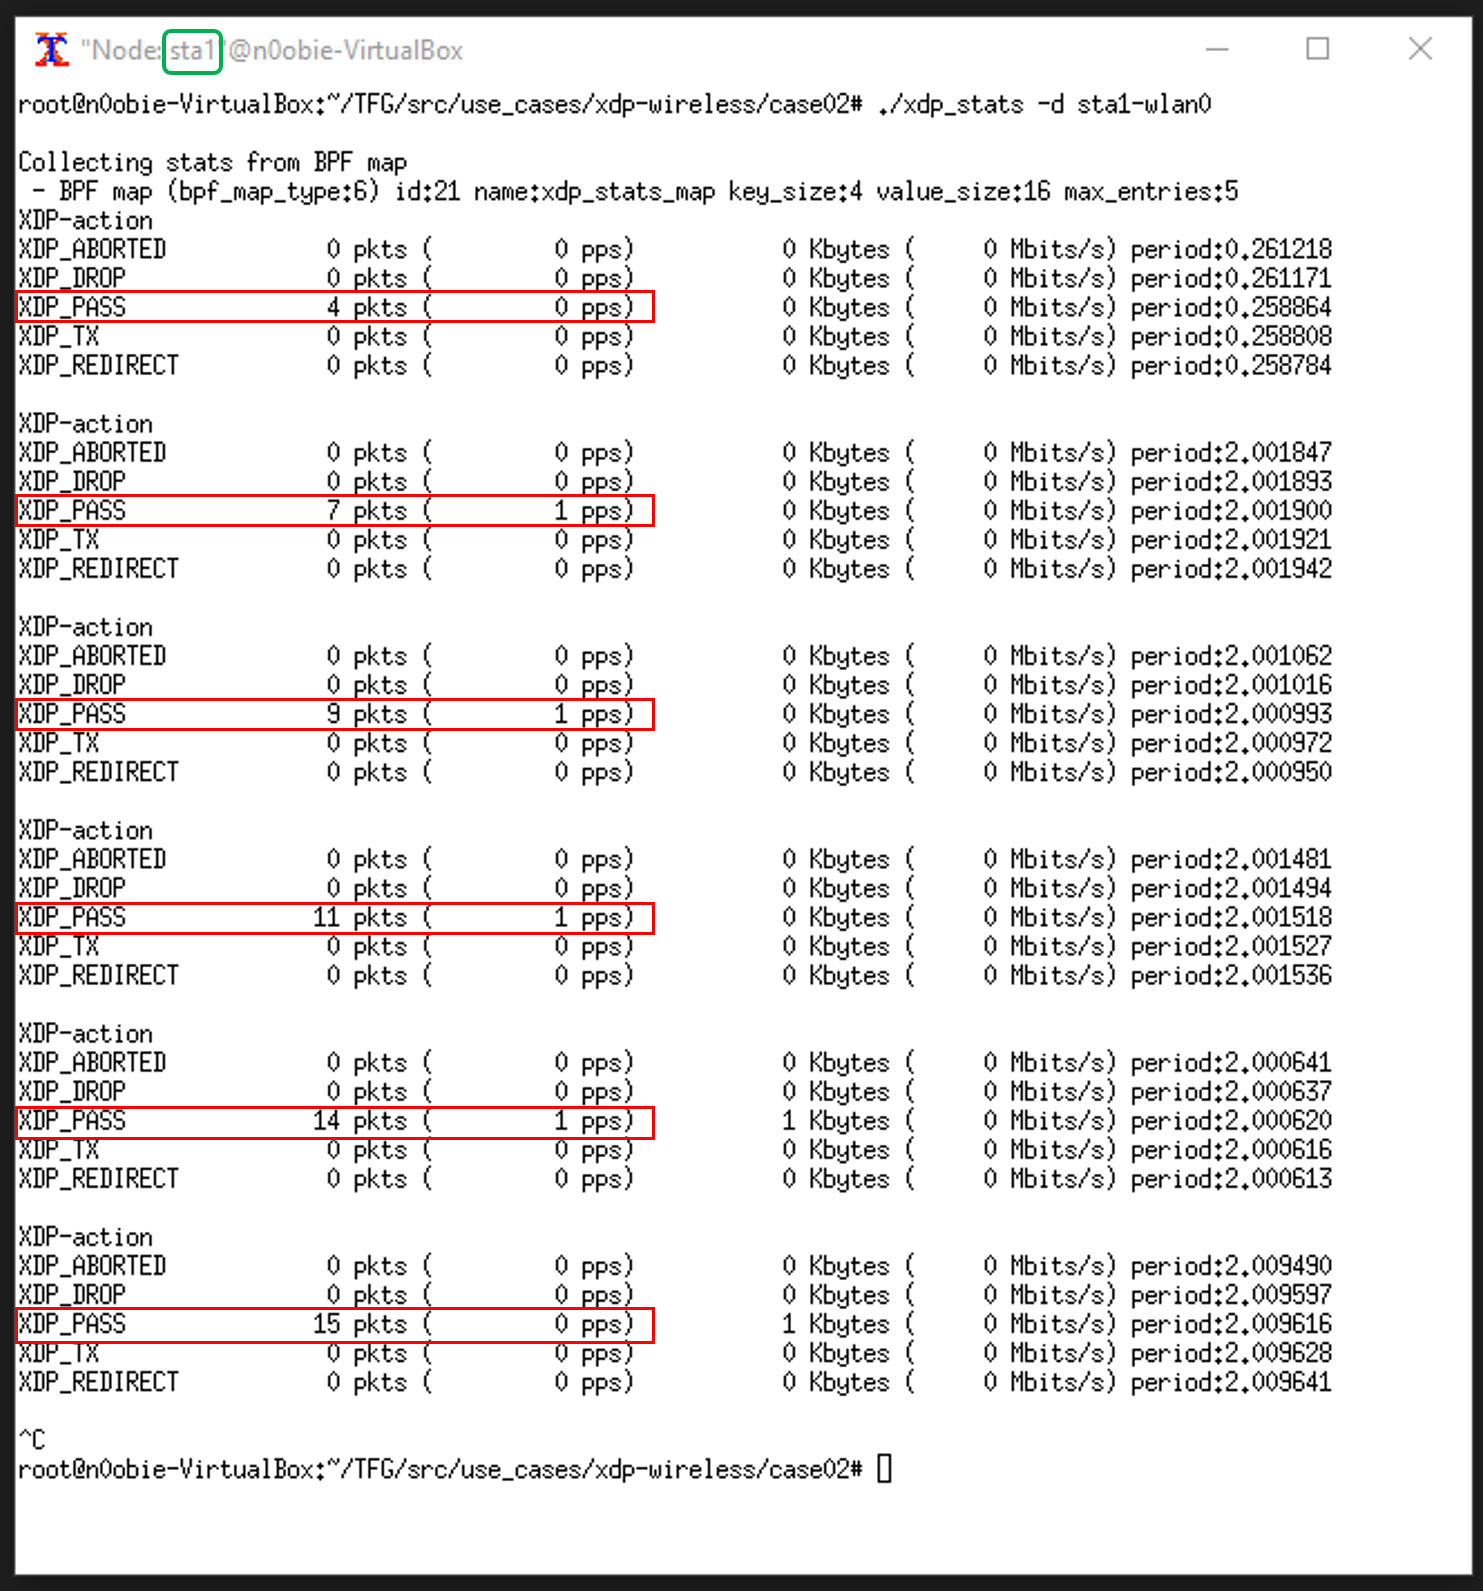
\includegraphics[width=14cm]{archivos/img/dev/xdp-wifi/case02/demo_case02_2_edited.png}
    \caption{Comprobación de funcionamiento (Stats) del Case02 - XDP Wireless}
    \label{fig:case02_xdp_wifi_func2}
\end{figure}

Según se puede ver en la figura \ref{fig:case02_xdp_wifi_func1}, hay perfecta conectividad entre las estaciones WiFi dado que el ping \fcolorbox{black}{green}{\rule{0pt}{2.5pt}\rule{2.5pt}{0pt}}\hspace{1mm} está funcionando correctamente. Por lo que, se presupone que el programa \gls{xdp} está dejando pasar los paquetes ICMP hacia el \textit{stack} de red. Apreciando la figura \ref{fig:case02_xdp_wifi_func1}, dicha presuposición se confirma, atendiendo al contador de los códigos de retorno \texttt{XDP\_PASS}. 